\section{Pasos en un proyecto de simulación}

\frame{\sectionpage}

\begin{frame}{Pasos en un proyecto de simulación}
    \begin{itemize}
        \item Hay un conjunto de pasos básicos para la realización de un proyecto de simulación.
        \item Tenga en cuenta que NO es un proceso secuencial.
        \item En ocasiones será necesario agregar o suprimir algunos pasos.
    \end{itemize}
\end{frame}

\begin{frame}{Metodología adaptada de \cite{BCN} and \cite{LK}}
    \begin{figure}
        \centering
        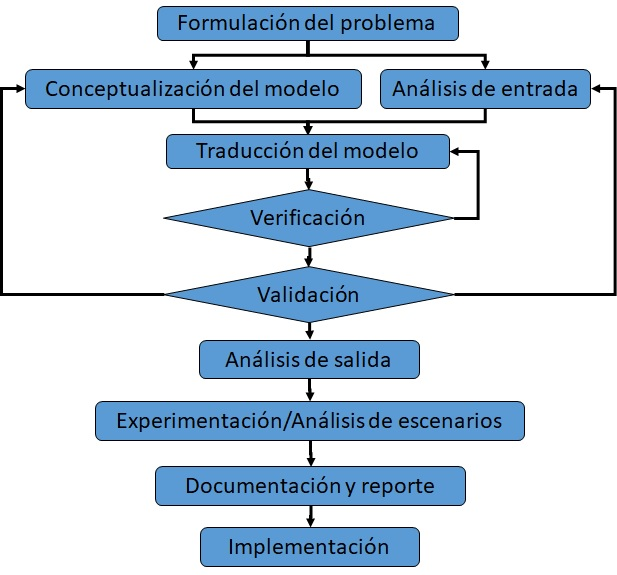
\includegraphics[width=7.5cm]{images/Metodologia.jpg}
        %\caption{Adaptado de \cite{BCN} and \cite{LK}}
        \label{fig:metodología}
    \end{figure}
\end{frame}

\begin{frame}{Formulación del problema}
    \begin{itemize}
        \item El estudio comienza con una declaración del problema.
        \item Se determinan los objetivos y el alcance del proyecto, se identifica al tomador de decisiones, al usuario y al modelista.
        \item Los objetivos indican las preguntas que serán respondidas.
    \end{itemize}
\end{frame}

\begin{frame}{Conceptualización del modelo}
    \begin{itemize}
        \item Se basa en la capacidad de abstraer los elementos esenciales del problema y sus interacciones.
        \item Emplea supuestos para caracterizar el sistema de forma básica y enriquecer el modelo hasta encontrar una aproximación útil.
    \end{itemize}
\end{frame}

\begin{frame}{Recolección de datos y análisis de entrada}
    \begin{itemize}
        \item Identificación, recolección y análisis de los datos necesarios para el estudio.
        \item Incluya datos del desempeño del sistema para validación.
    \end{itemize}
\end{frame}

\begin{frame}{Traducción del modelo}
    \begin{itemize}
        \item Se generan las instrucciones necesarias para lograr que el modelo pueda ser ejecutado en una computadora.
        \item Se debe decidir entre un lenguaje de programación general o un lenguaje de propósito específico.
    \end{itemize}
\end{frame}

\begin{frame}{Análisis de salida}
    \begin{itemize}
        \item Estimación de las medidas de desempeño del sistema y los diseños que están siendo simulados. 
        \item Se especifican los parámetros de corrida:
        \begin{enumerate}
            \item Número de réplicas independientes.
            \item Longitud de corrida.
            \item Longitud del periodo de calentamiento.
        \end{enumerate}
    \end{itemize}
\end{frame}

\begin{frame}{Experimentación y Análisis de escenarios}
    \begin{itemize}
        \item Determina las alternativas a evaluar con la simulación.
        \item Se comparan las alternativas en términos de las medidas de desempeño y costos.
    \end{itemize}
\end{frame}

\begin{frame}{Documentación y reporte}
    \begin{itemize}
        \item Reportar de forma clara y concisa en un documento:
        \begin{enumerate}
            \item Supuestos empleados.
            \item Análisis de resultados.
            \item Animación para comunicar los detalles del modelo.
            \item Discusión de la construcción del modelo y validación.
        \end{enumerate}
    \end{itemize}
\end{frame}